\documentclass[dvipdfmx]{jsarticle}
\setcounter{section}{2}
\setcounter{subsection}{1}
\usepackage{xr}
\externaldocument{8.1.1}
\externaldocument{8.1.2}
\externaldocument{8.1.3}
\externaldocument{8.1.5}
\externaldocument{8.2.1}
\usepackage{amsmath,amsfonts,amssymb,array,comment,mathtools,url,docmute}
\usepackage{longtable,booktabs,dcolumn,tabularx,mathtools,multirow,colortbl,xcolor}
\usepackage[dvipdfmx]{graphics}
\usepackage{bmpsize}
\usepackage{amsthm}
\usepackage{enumitem}
\setlistdepth{20}
\renewlist{itemize}{itemize}{20}
\setlist[itemize]{label=•}
\renewlist{enumerate}{enumerate}{20}
\setlist[enumerate]{label=\arabic*.}
\setcounter{MaxMatrixCols}{20}
\setcounter{tocdepth}{3}
\newcommand{\rotin}{\text{\rotatebox[origin=c]{90}{$\in $}}}
\newcommand{\amap}[6]{\text{\raisebox{-0.7cm}{\begin{tikzpicture} 
  \node (a) at (0, 1) {$\textstyle{#2}$};
  \node (b) at (#6, 1) {$\textstyle{#3}$};
  \node (c) at (0, 0) {$\textstyle{#4}$};
  \node (d) at (#6, 0) {$\textstyle{#5}$};
  \node (x) at (0, 0.5) {$\rotin $};
  \node (x) at (#6, 0.5) {$\rotin $};
  \draw[->] (a) to node[xshift=0pt, yshift=7pt] {$\textstyle{\scriptstyle{#1}}$} (b);
  \draw[|->] (c) to node[xshift=0pt, yshift=7pt] {$\textstyle{\scriptstyle{#1}}$} (d);
\end{tikzpicture}}}}
\newcommand{\twomaps}[9]{\text{\raisebox{-0.7cm}{\begin{tikzpicture} 
  \node (a) at (0, 1) {$\textstyle{#3}$};
  \node (b) at (#9, 1) {$\textstyle{#4}$};
  \node (c) at (#9+#9, 1) {$\textstyle{#5}$};
  \node (d) at (0, 0) {$\textstyle{#6}$};
  \node (e) at (#9, 0) {$\textstyle{#7}$};
  \node (f) at (#9+#9, 0) {$\textstyle{#8}$};
  \node (x) at (0, 0.5) {$\rotin $};
  \node (x) at (#9, 0.5) {$\rotin $};
  \node (x) at (#9+#9, 0.5) {$\rotin $};
  \draw[->] (a) to node[xshift=0pt, yshift=7pt] {$\textstyle{\scriptstyle{#1}}$} (b);
  \draw[|->] (d) to node[xshift=0pt, yshift=7pt] {$\textstyle{\scriptstyle{#2}}$} (e);
  \draw[->] (b) to node[xshift=0pt, yshift=7pt] {$\textstyle{\scriptstyle{#1}}$} (c);
  \draw[|->] (e) to node[xshift=0pt, yshift=7pt] {$\textstyle{\scriptstyle{#2}}$} (f);
\end{tikzpicture}}}}
\renewcommand{\thesection}{第\arabic{section}部}
\renewcommand{\thesubsection}{\arabic{section}.\arabic{subsection}}
\renewcommand{\thesubsubsection}{\arabic{section}.\arabic{subsection}.\arabic{subsubsection}}
\everymath{\displaystyle}
\allowdisplaybreaks[4]
\usepackage{vtable}
\theoremstyle{definition}
\newtheorem{thm}{定理}[subsection]
\newtheorem*{thm*}{定理}
\newtheorem{dfn}{定義}[subsection]
\newtheorem*{dfn*}{定義}
\newtheorem{axs}[dfn]{公理}
\newtheorem*{axs*}{公理}
\renewcommand{\headfont}{\bfseries}
\makeatletter
  \renewcommand{\section}{%
    \@startsection{section}{1}{\z@}%
    {\Cvs}{\Cvs}%
    {\normalfont\huge\headfont\raggedright}}
\makeatother
\makeatletter
  \renewcommand{\subsection}{%
    \@startsection{subsection}{2}{\z@}%
    {0.5\Cvs}{0.5\Cvs}%
    {\normalfont\LARGE\headfont\raggedright}}
\makeatother
\makeatletter
  \renewcommand{\subsubsection}{%
    \@startsection{subsubsection}{3}{\z@}%
    {0.4\Cvs}{0.4\Cvs}%
    {\normalfont\Large\headfont\raggedright}}
\makeatother
\makeatletter
\renewenvironment{proof}[1][\proofname]{\par
  \pushQED{\qed}%
  \normalfont \topsep6\p@\@plus6\p@\relax
  \trivlist
  \item\relax
  {
  #1\@addpunct{.}}\hspace\labelsep\ignorespaces
}{%
  \popQED\endtrivlist\@endpefalse
}
\makeatother
\renewcommand{\proofname}{\textbf{証明}}
\usepackage{tikz,graphics}
\usepackage[dvipdfmx]{hyperref}
\usepackage{pxjahyper}
\hypersetup{
 setpagesize=false,
 bookmarks=true,
 bookmarksdepth=tocdepth,
 bookmarksnumbered=true,
 colorlinks=false,
 pdftitle={},
 pdfsubject={},
 pdfauthor={},
 pdfkeywords={}}
\begin{document}
%\hypertarget{euclidux7a7aux9593}{%
\subsection{Euclid空間}%\label{euclidux7a7aux9593}}
%\hypertarget{euclidux7a7aux9593-1}{%
\subsubsection{Euclid空間}%\label{euclidux7a7aux9593-1}}
\begin{thm}\label{8.2.2.1} 次式のように写像$d_{E}$が定義されるとき、
\begin{align*}
d_{E}:\mathbb{R} \times \mathbb{R} \rightarrow \mathbb{R};(a,b) \mapsto |a - b|
\end{align*}
その組$\left( \mathbb{R},d_{E} \right)$は距離空間をなす。
\end{thm}
\begin{proof} 次式のように写像$d_{E}$が定義されるとき、
\begin{align*}
d_{E}:\mathbb{R} \times \mathbb{R} \rightarrow \mathbb{R};(a,b) \mapsto |a - b|
\end{align*}
$\forall a,b \in \mathbb{R}$に対し、$d(a,b) = |a - b| \geq 0$が成り立つかつ、$d(a,b) = |a - b| = 0$が成り立つならそのときに限り、$a = b$が成り立つかつ、$d(a,b) = |a - b| = |b - a| = d(b,a)$が成り立つことは明らかである。また、三角不等式より$\forall a,b,c \in \mathbb{R}$に対し、$d(a,c) = |a - c| \leq |a - b| + |b - c| = d(a,b) + d(b,c)$が成り立つ。以上より、その組$\left( \mathbb{R},d_{E} \right)$は距離空間をなす。
\end{proof}
\begin{dfn} 定理\ref{8.2.2.1}のような$n$つの距離空間$\left( \mathbb{R},d_{E} \right)$の直積距離空間を$n$次元Euclid空間といい、これを$E^{n}$と書く。さらに、その距離関数を$n$次元Euclid距離関数といい、ここでは、$d_{E^{n}}$と書くことにする。
\end{dfn}
\begin{thm}\label{8.2.2.2}
$n$次元Euclid距離関数$d_{E^{n}}$は$\mathbf{a} = \left( a_{i} \right)_{i \in \varLambda_{n}}$、$\mathbf{b} = \left( b_{i} \right)_{i \in \varLambda_{n}}$として次式のように与えられる。
\begin{align*}
d_{E^{n}}:\mathbb{R}^{n} \times \mathbb{R}^{n} \rightarrow \mathbb{R};\left( \mathbf{a},\mathbf{b} \right) \mapsto \sqrt{\sum_{i \in \varLambda_{n}} \left| a_{i} - b_{i} \right|^{2}}
\end{align*}
\end{thm}
\begin{proof} 直積距離空間の定義より明らかである。
\end{proof}
%\hypertarget{euclidux7a7aux9593ux306bux304aux3051ux308bux4f4dux76f8ux7a7aux9593ux306eux958bux57fa}{%
\subsubsection{Euclid空間における位相空間の開基}%\label{euclidux7a7aux9593ux306bux304aux3051ux308bux4f4dux76f8ux7a7aux9593ux306eux958bux57fa}}\par
$n$次元Euclid空間$E^{n}$の開基、基本近傍系について次の定理たちが有用であろう。
\begin{thm*}[定理\ref{8.2.1.4}の再掲]
距離空間$(S,d)$の開基として、開球体全体の集合$\mathfrak{U}$が挙げられる。
\end{thm*}
\begin{thm*}[定理\ref{8.2.1.6}の再掲]
距離空間$(S,d)$が与えられたとき、$\forall a \in S$に対し、その元$a$の基本近傍系として、その元$a$を中心とする開球体全体の集合$\mathfrak{U}_{a}$が挙げられる。
\end{thm*}\par
これにより、$\forall\mathbf{a} \in \mathbb{R}^{n}\forall V \in \mathbf{V}\left( \mathbf{a} \right)\exists B\left( \mathbf{a},\varepsilon \right) \in \mathfrak{U}_{\mathbf{a}}$に対し、次の図のように与えられる。
\begin{center}
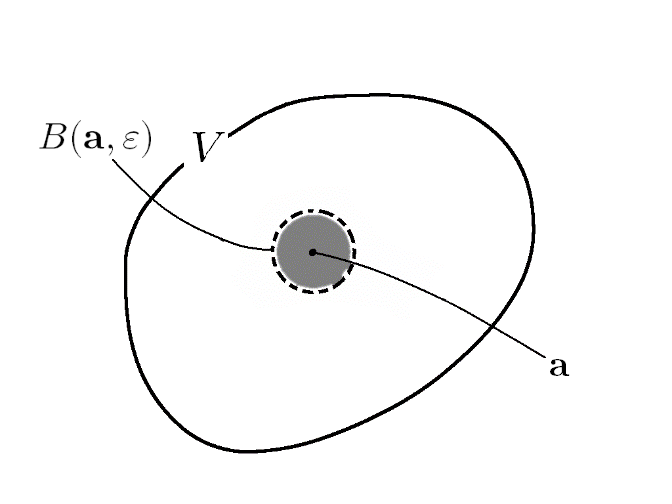
\includegraphics[width=60mm]{8.2.2.a.png}
\end{center}\par
ここで、特筆すべき$n$次元Euclid空間$E^{n}$の開基として次の定理たちのようなものがある。
\begin{thm}\label{8.2.2.3}
$n$次元Euclid空間$E^{n}$における位相空間$\left( \mathbb{R}^{n},\mathfrak{O}_{d_{E^{n}}} \right)$について、$\mathbf{a} \in \mathbb{R}^{n}$なる開球体$B\left( \mathbf{a},\varepsilon \right)$全体の集合$\mathfrak{B}$と、$\forall i \in \varLambda_{n}$に対し、$a_{i},b_{i} \in \mathbb{R}$が成り立つとき、直積$\prod_{i \in \varLambda_{n}} \left( a_{i},b_{i} \right)$全体の集合$\mathcal{I}$はどちらもその位相空間$\left( \mathbb{R}^{n},\mathfrak{O}_{d_{E^{n}}} \right)$の開基となる。
\end{thm}
\begin{proof}
$n$次元Euclid空間$E^{n}$における位相空間$\left( \mathbb{R}^{n},\mathfrak{O}_{d_{E^{n}}} \right)$について、$\mathbf{a} \in \mathbb{R}^{n}$なる開球$B\left( \mathbf{a},\varepsilon \right)$全体の集合$\mathfrak{B}$と、$\forall i \in \varLambda_{n}$に対し、$a_{i},b_{i} \in \mathbb{R}$が成り立つとき、直積$\prod_{i \in \varLambda_{n}} \left( a_{i},b_{i} \right)$全体の集合$\mathcal{I}$が与えられたとする。\par
このとき、$\forall O \in \mathfrak{O}_{d_{E^{n}}}\forall\mathbf{a} \in O$に対し、$\mathbf{a} = \left( a_{i} \right)_{i \in \varLambda_{n}}$とおくと、定義より明らかに$\mathbf{a} \in B\left( \mathbf{a},\varepsilon \right) \subseteq O$が成り立つような開球体$B\left( \mathbf{a},\varepsilon \right)$がその集合$\mathfrak{B}$に存在する。したがって、その集合$\mathfrak{B}$はその位相空間$\left( \mathbb{R}^{n},\mathfrak{O}_{d_{E^{n}}} \right)$の開基となる。\par
また、$\forall O \in \mathfrak{O}_{d_{E^{n}}}\forall\mathbf{a} \in O$に対し、定義より$\mathbf{a} \in B\left( \mathbf{a},\varepsilon \right) \subseteq O$が成り立つような開球体$B\left( \mathbf{a},\varepsilon \right)$が存在する。ここで、定理\ref{8.2.1.22}より次式が成り立つので、
\begin{align*}
\prod_{i \in \varLambda_{n}} {B\left( a_{i},\frac{\varepsilon}{\sqrt{n}} \right)} &= \prod_{i \in \varLambda_{n}} \left\{ b_{i} \in \mathbb{R} \middle| d_{E}\left( a_{i},b_{i} \right) < \frac{\varepsilon}{\sqrt{n}} \right\}\\
&= \prod_{i \in \varLambda_{n}} \left\{ b_{i} \in \mathbb{R} \middle| \left| a_{i} - b_{i} \right| < \frac{\varepsilon}{\sqrt{n}} \right\}\\
&= \prod_{i \in \varLambda_{n}} \left\{ b_{i} \in \mathbb{R} \middle| - \frac{\varepsilon}{\sqrt{n}} < a_{i} - b_{i} < \frac{\varepsilon}{\sqrt{n}} \right\}\\
&= \prod_{i \in \varLambda_{n}} \left\{ b_{i} \in \mathbb{R} \middle| a_{i} - \frac{\varepsilon}{\sqrt{n}} < b_{i} < a_{i} + \frac{\varepsilon}{\sqrt{n}} \right\}\\
&= \prod_{i \in \varLambda_{n}} \left( a_{i} - \frac{\varepsilon}{\sqrt{n}},a_{i} + \frac{\varepsilon}{\sqrt{n}} \right) \subseteq B\left( \mathbf{a},\varepsilon \right)
\end{align*}
$\forall O \in \mathfrak{O}_{d_{E^{n}}}\forall\mathbf{a} \in O\exists\prod_{i \in \varLambda_{n}} \left( a_{i} - \frac{\varepsilon}{\sqrt{n}},a_{i} + \frac{\varepsilon}{\sqrt{n}} \right)\in \mathcal{I}$に対し、$\mathbf{a} \in \prod_{i \in \varLambda_{n}} \left( a_{i} - \frac{\varepsilon}{\sqrt{n}},a_{i} + \frac{\varepsilon}{\sqrt{n}} \right) \subseteq O$が成り立ち、したがって、その集合$\mathcal{I}$はその位相空間$\left( \mathbb{R}^{n},\mathfrak{O}_{d_{E^{n}}} \right)$の開基となる。
\end{proof}
\begin{thm}\label{8.2.2.4}
さらに、$n$次元Euclid空間$E^{n}$における位相空間$\left( \mathbb{R}^{n},\mathfrak{O}_{d_{E^{n}}} \right)$について、$\mathbf{a}' \in \mathbb{R}^{n}$なる開球体$B\left( \mathbf{a}',r \right)$のうち、$\mathbf{a}' \in \mathbb{Q}^{n}$かつ$r \in \mathbb{Q}$を満たすもの全体の集合$\mathfrak{B}'$もまたその位相空間$\left( \mathbb{R}^{n},\mathfrak{O}_{d_{E^{n}}} \right)$の開基となる。
\end{thm}\par
これは次の図のように考えられることで示される。
\begin{center}
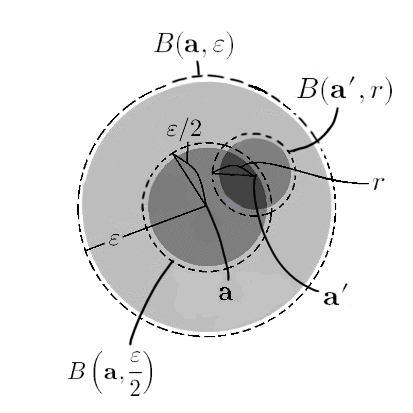
\includegraphics[width=60mm]{8.2.2.b.png}
\end{center}
\begin{proof}
$n$次元Euclid空間$E^{n}$における位相空間$\left( \mathbb{R}^{n},\mathfrak{O}_{d_{E^{n}}} \right)$について、$\mathbf{a}' \in \mathbb{R}^{n}$なる開球$B\left( \mathbf{a}',r \right)$のうち、$\mathbf{a}' \in \mathbb{Q}^{n}$かつ$r \in \mathbb{Q}$を満たすもの全体の集合$\mathfrak{B}'$が与えられたとする。\par
$\forall O \in \mathfrak{O}_{d_{E^{n}}}\forall\mathbf{a} \in O$に対し、定義より明らかに$\mathbf{a} \in B\left( \mathbf{a},\varepsilon \right) \subseteq O$が成り立つような開球体$B\left( \mathbf{a},\varepsilon \right)$がその集合$\mathfrak{B}$に存在する。ここで、開球体$B\left( \mathbf{a},\frac{\varepsilon}{2} \right)$の$\mathbf{a}' \in \mathbb{Q}^{n}$なる元$\mathbf{a}'$がとられ、さらに、有理数の稠密性より$d_{E^{n}}\left( \mathbf{a},\mathbf{a}' \right) < r < \frac{\varepsilon}{2}$なる有理数$r$もとられることができるで、$B\left( \mathbf{a}',r \right) \subseteq B\left( \mathbf{a},\varepsilon \right)$が成り立つ。これにより、$\forall O \in \mathfrak{O}_{d_{E^{n}}}\forall\mathbf{a} \in O\exists B\left( \mathbf{a}',\varepsilon \right) \in \mathfrak{B}'$に対し、$\mathbf{a} \in B\left( \mathbf{a}',r \right) \subseteq O$が成り立ち、したがって、その集合$\mathfrak{B}'$はその位相空間$\left( \mathbb{R}^{n},\mathfrak{O}_{d_{E^{n}}} \right)$の開基となる。
\end{proof}
\begin{thm}\label{8.2.2.5}
その位相空間$\left( \mathbb{R}^{n},\mathfrak{O}_{d_{E^{n}}} \right)$は第2可算公理を満たす。
\end{thm}
\begin{proof} 定理\ref{8.2.2.4}での開基$\mathfrak{B}'$を用いて${\#}\mathfrak{B}' = {\#}\left( \mathbb{Q}^{n} \times \mathbb{Q} \right) = \aleph_{0}$が成り立つことによる。
\end{proof}
%\hypertarget{euclidux7a7aux9593ux306bux304aux3051ux308bux4f4dux76f8ux7a7aux9593ux306eux9023ux7d9aux5199ux50cf}{%
\subsubsection{Euclid空間における位相空間の連続写像}%\label{euclidux7a7aux9593ux306bux304aux3051ux308bux4f4dux76f8ux7a7aux9593ux306eux9023ux7d9aux5199ux50cf}}
\begin{dfn}
ここで、詳しくは解析学のほうに参照してもらいたいが、1つの位相空間$\left( S,\mathfrak{O} \right)$が与えられ写像$f:S \rightarrow \mathbb{R}^{n}$がその位相空間$\left( S,\mathfrak{O} \right)$から$n$次元Euclid空間$E^{n}$における位相空間$\left( \mathbb{R}^{n},\mathfrak{O}_{d_{E^{n}}} \right)$への連続写像であるとき、その写像$f$は実連続関数であるともいう。
\end{dfn}
\begin{thm}\label{8.2.2.6}
ここで、1つの位相空間$\left( S,\mathfrak{O} \right)$が与えられ写像$f:S \rightarrow \mathbb{R}$について、次のことは同値である。
\begin{itemize}
\item
  その写像$f$がその位相空間$\left( S,\mathfrak{O} \right)$から1次元Euclid空間$E$における位相空間$\left( \mathbb{R},\mathfrak{O}_{d_{E}} \right)$への連続写像である。
\item
  $\forall a,b \in \mathbb{R}$に対し、開区間$(a,b)$に制限されたその逆対応$f^{- 1}$の値域$V\left( f^{- 1}|(a,b) \right)$がその位相$\mathfrak{O}$に属する。
\item
  $\forall c \in \mathbb{R}$に対し、開区間たち$(c,\infty)、( - \infty,c)$に制限されたその逆対応$f^{- 1}$の値域たち$V\left( f^{- 1}|(c,\infty) \right)$、$V\left( f^{- 1}|( - \infty,c) \right)$がその位相$\mathfrak{O}$に属する。
\end{itemize}
\end{thm}
\begin{proof}
1つの位相空間$\left( S,\mathfrak{O} \right)$が与えられ写像$f:S \rightarrow \mathbb{R}$について、その写像$f$がその位相空間$\left( S,\mathfrak{O} \right)$から1次元Euclid空間$E$における位相空間$\left( \mathbb{R},\mathfrak{O}_{d_{E}} \right)$への連続写像であるとする。このとき、開区間$(a,b)$全体の集合$\mathcal{I}$は定理\ref{8.2.2.3}よりその位相空間$\left( \mathbb{R},\mathfrak{O}_{d_{E}} \right)$の開基となり、したがって、準開基でもあるのであった。定理\ref{8.1.3.2}よりその写像$f:S \rightarrow \mathbb{R}$が連続であるならそのときに限り、$\forall I\in \mathcal{I}$に対し、$V\left( f^{- 1} \middle| I \right)\in \mathfrak{O}$が成り立つことになる、即ち、$\forall a,b \in \mathbb{R}$に対し、開区間$(a,b)$に制限されたその逆対応$f^{- 1}$の値域$V\left( f^{- 1}|(a,b) \right)$がその位相$\mathfrak{O}$に属することになる。\par
さらに、その集合$\mathfrak{U}$の任意の元は開区間で任意の開区間$(a,b)$は$(a,b) = (a,\infty) \cap ( - \infty,b)$のように書き換えられることができるので、定義より明らかに$c \in \mathbb{R}$なる開区間たち$(c,\infty)$、$( - \infty,c)$全体の集合$\mathcal{I}'$はその位相空間$\left( \mathbb{R},\mathfrak{O}_{d_{E}} \right)$の開基となり、したがって、準開基でもある。ここで、定理\ref{8.1.3.2}よりその写像$f:S \rightarrow \mathbb{R}$が連続であるならそのときに限り、$\forall I \in \mathcal{I}'$に対し、$V\left( f^{- 1} \middle| I \right)\in \mathfrak{O}$が成り立つことになる、即ち、$\forall c \in D$に対し、開区間たち$(c,\infty)$、$( - \infty,c)$に制限されたその逆対応$f^{- 1}$の値域たち$V\left( f^{- 1}|(c,\infty) \right)$、$V\left( f^{- 1}|( - \infty,c) \right)$がその位相$\mathfrak{O}$に属することになる。
\end{proof}
\begin{thm}\label{8.2.2.7}
1つの位相空間$\left( S,\mathfrak{O} \right)$と$n$次元Euclid空間$E^{n}$が与えられたとき、写像$f:S \rightarrow \mathbb{R}^{n}$が連続であるならそのときに限り、$\forall a \in S\forall\varepsilon \in \mathbb{R}^{+}$に対し、これのある近傍$V$をとれば、$\forall b \in V$に対し、$d_{E^{n}}\left( f(a),f(b) \right) < \varepsilon$が成り立つ。
\end{thm}\par
特に、その位相空間$\left( S,\mathfrak{O} \right)$が$m$次元Euclid空間$E^{m}$における位相空間であるなら、定理\ref{8.2.1.14}より$\forall\varepsilon \in \mathbb{R}^{+}\exists\delta \in \mathbb{R}^{+}\forall b \in \mathbb{R}^{m}$に対し、$d_{E^{m}}(a,b) < \delta$なら$d_{E^{n}}\left( f(a),f(b) \right) < \varepsilon$が成り立つ。この式はいわゆる$\varepsilon $-$\delta $論法の式である。
\begin{proof}
1つの位相空間$\left( S,\mathfrak{O} \right)$と$n$次元Euclid空間$E^{n}$が与えられたとき、$\forall\mathbf{a} \in \mathbb{R}^{n}$に対し、その元を中心とする開球体全体の集合$\mathfrak{U}_{\mathbf{a}}$は定理\ref{8.2.1.6}よりその元$\mathbf{a}$のその$n$次元Euclid空間における位相空間$\left( \mathbb{R}^{n},\mathfrak{O}_{d_{E^{n}}} \right)$における基本近傍系となり、したがって、全近傍系となるのであった。\par
ここで、定理\ref{8.1.3.1}より写像$f:S \rightarrow \mathbb{R}^{n}$が連続であるならそのときに限り、$a \in S$かつ$\mathbf{a} \in \mathbb{R}^{n}$なる元々$a$、$\mathbf{a}$のそれらの位相空間たち$\left( S,\mathfrak{O} \right)$、$\left( \mathbb{R}^{n},\mathfrak{O}_{d_{E^{n}}} \right)$の全近傍系たちがそれぞれ$\mathbf{V}(a)$、$\mathfrak{U}_{\mathbf{a}}$とおかれると、$B\left( f(a),\varepsilon \right) \in \mathfrak{U}_{f(a)}$なら$V\left( f^{- 1}|B\left( f(a),\varepsilon \right) \right) \in \mathbf{V}(a)$が成り立つ。ここで、$V\left( f^{- 1}|B\left( f(a),\varepsilon \right) \right) \in \mathbf{V}(a)$について、$B\left( f(a),\varepsilon \right) \in \mathfrak{U}_{f(a)}$が成り立つかつ、その写像$f$が連続であるので、$V\left( f^{- 1}|B\left( f(a),\varepsilon \right) \right)\in \mathfrak{O}$が成り立つことに注意すれば、次のようになる。
\begin{align*}
V\left( f^{- 1}|B\left( f(a),\varepsilon \right) \right) \in \mathbf{V}(a) &\Leftrightarrow a \in {\mathrm{int}}{V\left( f^{- 1}|B\left( f(a),\varepsilon \right) \right)}\\
&\Leftrightarrow a \in V\left( f^{- 1}|B\left( f(a),\varepsilon \right) \right)\\
&\Leftrightarrow a \in \left\{ b \in S \middle| \exists a' \in B\left( f(a),\varepsilon \right)\left[ f(b) = a' \right] \right\}\\
&\Leftrightarrow a \in \left\{ b \in S \middle| f(b) \in B\left( f(a),\varepsilon \right) \right\}\\
&\Leftrightarrow a \in \left\{ b \in S \middle| d_{E^{n}}\left( f(a),f(b) \right) < \varepsilon \right\}
\end{align*}
ここで、その値域$V\left( f^{- 1}|B\left( f(a),\varepsilon \right) \right)$を$V$とおくと、$\forall b \in V$に対し、次式が成り立つ。
\begin{align*}
d_{E^{n}}\left( f(a),f(b) \right) < \varepsilon
\end{align*}\par
以上より、その写像$f:S \rightarrow \mathbb{R}^{n}$が連続であるならそのときに限り、$\forall a \in S\forall\varepsilon \in \mathbb{R}^{+}$に対し、これのある近傍$V$をとれば、$\forall b \in V$に対し、$d_{E^{n}}\left( f(a),f(b) \right) < \varepsilon$が成り立つ。
\end{proof}
\begin{thm}\label{8.2.2.8}
1つの位相空間$\left( S,\mathfrak{O} \right)$と$n$次元Euclid空間$E^{n}$が与えられたとき、写像たち$f:S \rightarrow \mathbb{R}^{n}$、$g:S \rightarrow \mathbb{R}^{n}$が連続であるなら、$\forall a,b \in \mathbb{R}$に対し、その写像$af + bg$も連続で、特に、$n = 1$のとき、写像たち$fg$、$\frac{f}{g}$も連続である\footnote{実いうと、$n = 2$のとき、$\mathbb{C} =\mathbb{R}^2 $と考えれば、複素数の積の定義より複素数同士の積や商はそれぞれ実数の和積、和積と商で書かれることができるので、$n = 2$のときでも写像たち$fg$、$\frac{f}{g}$も連続となります。}。
\end{thm}
\begin{proof}
1つの位相空間$\left( S,\mathfrak{O} \right)$と$n$次元Euclid空間$E^{n}$が与えられたとき、写像たち$f:S \rightarrow \mathbb{R}^{n}$、$g:S \rightarrow \mathbb{R}^{n}$が連続であるなら、$\forall s \in S\forall\varepsilon \in \mathbb{R}^{+}$に対し、これのある近傍たち$V$、$W$をとれば、$\forall v \in V\forall w \in W$に対し、次式が成り立つ。
\begin{align*}
d_{E^{n}}\left( f(s),f(v) \right) < \varepsilon,\ \ d_{E^{n}}\left( g(s),g(w) \right) < \varepsilon
\end{align*}
特に、$\forall v \in V \cap W$に対し、次式が成り立つ。
\begin{align*}
d_{E^{n}}\left( f(s),f(v) \right) < \varepsilon,\ \ d_{E^{n}}\left( g(s),g(v) \right) < \varepsilon
\end{align*}
ここで、$\forall a,b \in \mathbb{R}$に対し、$a = b = 0$のときは明らかであるから、$a \neq 0$または$b \neq 0$のとき、次のようになる。
\begin{align*}
d_{E^{n}}\left( (af + bg)(s),(af + bg)(v) \right) &= d_{E^{n}}\left( af(s) + bg(s),af(v) + bg(v) \right)\\
&= d_{E^{n}}\left( af(s) - af(v),bg(s) - bg(v) \right)\\
&\leq d_{E^{n}}\left( af(s) - af(v),0 \right) + d_{E^{n}}\left( bg(s) - bg(v),0 \right)\\
&= d_{E^{n}}\left( af(s),af(v) \right) + d_{E^{n}}\left( bg(s),bg(v) \right)\\
&= |a|d_{E^{n}}\left( f(s),f(v) \right) + |b|d_{E^{n}}\left( g(s),g(v) \right)\\
&< |a|\varepsilon + |b|\varepsilon = \left( |a| + |b| \right)\varepsilon
\end{align*}
定理\ref{8.2.2.7}よりその写像$af + bg$も連続である。\par
特に、$n = 1$のとき、次のようになる。
\begin{align*}
d_{E}\left( fg(s),fg(v) \right) &= d_{E}\left( f(s)g(s),f(v)g(v) \right)\\
&= d_{E}\left( f(s)g(s) + f(s)g(v) - f(s)g(v),f(v)g(v) \right)\\
&= d_{E}\left( f(s)g(s) - f(s)g(v), - f(s)g(v) + f(v)g(v) \right)\\
&= d_{E}\left( f(s)\left( g(s) - g(v) \right), - g(v)\left( f(s) - f(v) \right) \right)\\
&\leq d_{E}\left( f(s)\left( g(s) - g(v) \right),0 \right) + d_{E}\left( - g(v)\left( f(s) - f(v) \right),0 \right)\\
&= d_{E}\left( f(s),0 \right)d_{E}\left( g(s) - g(v),0 \right) + d_{E}\left( g(v),0 \right)d_{E}\left( f(s) - f(v),0 \right)\\
&= d_{E}\left( f(s),0 \right)d_{E}\left( g(s),g(v) \right) + d_{E}\left( g(v),0 \right)d_{E}\left( f(s),f(v) \right)\\
&\leq \left( d_{E}\left( f(s),f(v) \right) + d_{E}\left( f(v),0 \right) \right)d_{E}\left( g(s),g(v) \right) + d_{E}\left( g(v),0 \right)d_{E}\left( f(s),f(v) \right)\\
&< \left( \varepsilon + d_{E}\left( f(v),0 \right) \right)\varepsilon + d_{E}\left( g(v),0 \right)\varepsilon\\
&= \left( \varepsilon + d_{E}\left( f(v),0 \right) + d_{E}\left( g(v),0 \right) \right)\varepsilon
\end{align*}
定理\ref{8.2.2.7}よりその写像$fg$も連続である。\par
また、$0 < \varepsilon < \frac{1}{2}d_{E}\left( g(v),0 \right)$とおかれれば、$d_{E}\left( g(s),g(v) \right) < \varepsilon < \frac{1}{2}d_{E}\left( g(v),0 \right)$が成り立ち、したがって、次のようになる。
\begin{align*}
\frac{1}{2}d_{E}\left( g(v),0 \right) &= d_{E}\left( g(v),0 \right) - \frac{1}{2}d_{E}\left( g(v),0 \right)\\
&< d_{E}\left( g(v),0 \right) - \varepsilon\\
&= d_{E}\left( g(v),0 \right) - d_{E}\left( g(s),0 \right) + d_{E}\left( g(s),0 \right) - \varepsilon\\
&\leq d_{E}\left( g(v),g(s) \right) + d_{E}\left( g(s),0 \right) - d_{E}\left( g(s),0 \right) + d_{E}\left( g(s),0 \right) - \varepsilon\\
&= d_{E}\left( g(v),g(s) \right) + d_{E}\left( g(s),0 \right) - \varepsilon\\
&< \varepsilon + d_{E}\left( g(s),0 \right) - \varepsilon\\
&= d_{E}\left( g(s),0 \right)
\end{align*}
これにより、次のようになる。
\begin{align*}
d_{E}\left( \frac{1}{g(s)},\frac{1}{g(v)} \right) &= d_{E}\left( \frac{1}{g(s)} - \frac{1}{g(v)},0 \right)\\
&= d_{E}\left( \frac{g(v) - g(s)}{g(s)g(v)},0 \right)\\
&= \frac{d_{E}\left( g(v) - g(s),0 \right)}{d_{E}\left( g(s),0 \right)d_{E}\left( g(v),0 \right)}\\
&= \frac{d_{E}\left( g(s),g(v) \right)}{d_{E}\left( g(s),0 \right)d_{E}\left( g(v),0 \right)}\\
&< \frac{\varepsilon}{\frac{1}{2}{d_{E}\left( g(v),0 \right)}^{2}}
\end{align*}
定理\ref{8.2.2.7}よりその写像$\frac{f}{g}$も連続である。
\end{proof}
\begin{thm}\label{8.2.2.9}
距離空間$(S,d)$が与えられたとき、その距離関数$d$がその距離空間$(S,d)$の直積距離空間$\left( S \times S,d' \right)$における位相空間$\left( S \times S,\mathfrak{O}_{d'} \right)$から1次元Euclid空間$E$における位相空間$\left( \mathbb{R},\mathfrak{O}_{d_{E}} \right)$への連続写像である。
\end{thm}
\begin{proof}
距離空間$(S,d)$が与えられたとき、直積$S \times S$の元の列$\left( a_{n},b_{n} \right)_{n \in \mathbb{N}}$が極限をもつとすれば、定理\ref{8.2.1.24}より次式が成り立つので、
\begin{align*}
\lim_{n \rightarrow \infty}{d\left( a_{n},b_{n} \right)} = d\left( \lim_{n \rightarrow \infty}a_{n},\lim_{n \rightarrow \infty}b_{n} \right)
\end{align*}
定理\ref{8.2.1.14}よりその距離関数$d$がその距離空間$(S,d)$の直積距離空間$\left( S \times S,d' \right)$における位相空間$\left( S \times S,\mathfrak{O}_{d'} \right)$から1次元Euclid空間$E$における位相空間$\left( \mathbb{R},\mathfrak{O}_{d_{E}} \right)$への連続写像である。
\end{proof}
\begin{thm}\label{8.2.2.10}
1次元Euclid空間$E$における位相空間$\left( \mathbb{R},\mathfrak{O}_{d_{E}} \right)$は、$\forall a,b \in \mathbb{R}$に対し、開区間$(a,b)$を台集合とする部分位相空間$\left( (a,b),\left( \mathfrak{O}_{d_{E}} \right)_{(a,b)} \right)$と同相である。
\end{thm}
\begin{proof}
1次元Euclid空間$E$における位相空間$\left( \mathbb{R},\mathfrak{O}_{d_{E}} \right)$について、$\forall a,b \in \mathbb{R}$に対し、開区間$(a,b)$を台集合とする部分位相空間$\left( (a,b),\left( \mathfrak{O}_{d_{E}} \right)_{(a,b)} \right)$が与えられたとき、次のような写像$f$が考えられれば、
\begin{align*}
f&:( - 1,1) \rightarrow \mathbb{R};x \mapsto \frac{x}{1 - x^{2}}\\
g&:(a,b) \rightarrow ( - 1,1);x \mapsto \frac{2}{b - a}\left( x - \frac{a + b}{2} \right)
\end{align*}
その合成写像$f \circ g$がこれらの位相空間たち$\left( \mathbb{R},\mathfrak{O}_{d_{E}} \right)$、$\left( (a,b),\left( \mathfrak{O}_{d_{E}} \right)_{(a,b)} \right)$の間の同相写像となる。
\end{proof}
%\hypertarget{euclidux7a7aux9593ux306bux304aux3051ux308bux4f4dux76f8ux7a7aux9593ux306eux9023ux7d50}{%
\subsubsection{Euclid空間における位相空間の連結}%\label{euclidux7a7aux9593ux306bux304aux3051ux308bux4f4dux76f8ux7a7aux9593ux306eux9023ux7d50}}
\begin{thm}\label{8.2.2.11}
1次元Euclid空間$E$における位相空間$\left( \mathbb{R},\mathfrak{O}_{d_{E}} \right)$について、$\forall a,b \in \mathbb{R}$に対し、次の集合たちを台集合とする部分位相空間はいづれも連結である。
\begin{align*}
\mathbb{R},\ \ (a,b),\ \ [ a,b]&,\ \ (a,b],\ \ [ a,b), \\ 
(a,\infty),\ \ [ a,\infty),\ \ &( - \infty,b),\ \ ( - \infty,b]
\end{align*}
\end{thm}
\begin{proof}
1次元Euclid空間$E$における位相空間$\left( \mathbb{R},\mathfrak{O}_{d_{E}} \right)$について、空集合でない2つの閉集合たち$A$、$B$を用いて$\mathbb{R} = A \sqcup B$が成り立つと仮定しよう。これらの閉集合たちの実数たちそれぞれ$a$、$b$がとられれば、$a \neq b$が成り立つので、$a < b$としても一般性は失われなくそうする。このとき、$a \in A \cap ( - \infty,b)$が成り立つので、$A \cap ( - \infty,b) \neq \emptyset$が成り立つ。また、その実数$b$がその集合$A \cap ( - \infty,b)$の1つの上界であるから、その集合$A \cap ( - \infty,b)$の上限$c$が存在して$c = \sup\left( A \cap ( - \infty,b) \right) \leq b$が成り立ち、したがって、$\forall\varepsilon \in \mathbb{R}^{+}$に対し、$c - \varepsilon < a' \leq c$なる実数$a'$がその集合$A \cap ( - \infty,b)$に、したがって、その集合$A$に存在するので、$(c - \varepsilon,c + \varepsilon) \cap A \neq \emptyset$が成り立つ、即ち、$B(c,\varepsilon) \cap A \neq \emptyset$が成り立つ。ここで、定理\ref{8.1.2.17}と定理\ref{8.2.1.9}より$c \in {\mathrm{cl}}A = A$が成り立つ。これにより、$c < b$が成り立つ。一方で、$c = \sup\left( A \cap ( - \infty,b) \right) < d \leq b$なる実数$d$が$d \in A$を満たすとすれば、$d \neq b$が成り立つので、$d \in A \cap ( - \infty,b)$が成り立つことになるが、これは上限の定義に矛盾している。したがって、$d \in \mathbb{R} \setminus A = B$が成り立つ。このとき、$\forall\varepsilon \in \mathbb{R}^{+}$に対し、$d \in (c - \varepsilon,c + \varepsilon)$が成り立つので、$(c - \varepsilon,c + \varepsilon) \cap B \neq \emptyset$が成り立つ、即ち、$B(c,\varepsilon) \cap B \neq \emptyset$が成り立つ。ここで、定理\ref{8.1.2.17}と定理\ref{8.2.1.9}より$c \in {\mathrm{cl}}B = B$が成り立つ。これにより、$c \in A \cap B$が成り立つことになるが、これは仮定に矛盾している。したがって、空集合でない任意の2つの閉集合たち$A$、$B$は$\mathbb{R} = A \sqcup B$を満たせない。したがって、定理\ref{8.1.5.1}より1次元Euclid空間$E$における位相空間$\left( \mathbb{R},\mathfrak{O}_{d_{E}} \right)$は連結である。\par
また、$\forall a,b \in \mathbb{R}$に対し、その部分位相空間$\left( (a,b),\left( \mathfrak{O}_{d_{E}} \right)_{(a,b)} \right)$は定理\ref{8.2.2.10}より連結である。さらに、定理\ref{8.1.5.5}より$\forall a,b \in \mathbb{R}$に対し、次の集合たちを台集合とする部分位相空間はいづれも連結である。
\begin{align*}
[ a,b],\ \ (a,b],\ \ [ a,b)
\end{align*}
最後に、定理\ref{8.1.5.7}より$\forall a,b \in \mathbb{R}$に対し、次式のようにおかれれば、
\begin{align*}
(a,\infty) = \bigcup_{n \in \mathbb{N}} (a,a + n)&,\ \ [ a,\infty) = \bigcup_{n \in \mathbb{N}} [ a,a + n),\\ 
( - \infty,b) = \bigcup_{n \in \mathbb{N}} (b - n,b)&,\ \ ( - \infty,b] = \bigcup_{n \in \mathbb{N}} (b - n,b]
\end{align*}
次の集合たちを台集合とする部分位相空間はいづれも連結である。
\begin{align*}
(a,\infty),\ \ [ a,\infty),\ \ ( - \infty,b),\ \ ( - \infty,b]
\end{align*}\par
以上、$\forall a,b \in \mathbb{R}$に対し、上記の集合たちを台集合とする部分位相空間はいづれも連結であることが示された。
\end{proof}
\begin{thm}\label{8.2.2.12}
$n$次元Euclid空間$E^{n}$における位相空間$\left( \mathbb{R}^{n},\mathfrak{O}_{d_{E^{n}}} \right)$は連結である。
\end{thm}
\begin{proof} 定理\ref{8.1.5.11}と定理\ref{8.2.2.11}より明らかである。
\end{proof}
\begin{thm}\label{8.2.2.13}
1次元Euclid空間$E$における位相空間$\left( \mathbb{R},\mathfrak{O}_{d_{E}} \right)$の連結な部分位相空間$\left( M,\mathfrak{O}_{M} \right)$が与えられたとき、$\forall a,b \in M$に対し、$a < b$が成り立つなら、$[ a,b] \subseteq M$が成り立つ。
\end{thm}
\begin{proof}
1次元Euclid空間$E$における位相空間$\left( \mathbb{R},\mathfrak{O}_{d_{E}} \right)$の連結な部分位相空間$\left( M,\mathfrak{O}_{M} \right)$が与えられたとする。$M = \left\{ a \right\}$が成り立つなら、$M = [ a,a]$が成り立つので、その部分集合$M$はこれの元を2つ以上もつとしてもよい。ここで、$\exists a,b \in M$に対し、$a < b$が成り立つかつ、$[ a,b] \subseteq M$が成り立たないと仮定する。このとき、$\exists c \in [ a,b]$に対し、$c \notin M$が成り立ち、したがって、次式が成り立つ。
\begin{align*}
M = M \setminus \left\{ c \right\} \subseteq \mathbb{R} \setminus \left\{ c \right\} = ( - \infty,c) \cup (c,\infty),\ \ ( - \infty,c) \cap (c,\infty) \cap M \subseteq ( - \infty,c) \cap (c,\infty) = \emptyset
\end{align*}
さらに、$a,b \in M$かつ$a \in ( - \infty,c)$かつ$b \in (c,\infty)$が成り立つので、$( - \infty,c) \cap M \neq \emptyset$かつ$(c,\infty) \cap M \neq \emptyset$が成り立つ。このとき、集合たち$( - \infty,c)$、$(c,\infty)$はいづれも開集合であり、次式が成り立つ。
\begin{align*}
M \subseteq ( - \infty,c) \cup (c,\infty)&,\ \ ( - \infty,c) \cap (c,\infty) \cap M = \emptyset,\\
( - \infty,c) \cap M \neq \emptyset&,\ \ (c,\infty) \cap M \neq \emptyset
\end{align*}
ここで、定理\ref{8.1.5.2}よりその位相空間$\left( \mathbb{R},\mathfrak{O}_{d_{E}} \right)$が連結でないことになるが、これは仮定に矛盾している。したがって、$\forall a,b \in M$に対し、$a < b$が成り立つなら、$[ a,b] \subseteq M$が成り立つ。
\end{proof}
\begin{thm}\label{8.2.2.14}
1次元Euclid空間$E$における位相空間$\left( \mathbb{R},\mathfrak{O}_{d_{E}} \right)$について、$\forall a,b \in \mathbb{R}$に対し、次の集合たちを台集合とする部分位相空間以外で連結な部分位相空間は存在しない。
\begin{align*}
\mathbb{R},\ \ (a,b),\ \ [ a,b]&,\ \ (a,b],\ \ [ a,b),\\ 
(a,\infty),\ \ [ a,\infty),\ \ &( - \infty,b),\ \ ( - \infty,b]
\end{align*}
\end{thm}
\begin{proof}
1次元Euclid空間$E$における位相空間$\left( \mathbb{R},\mathfrak{O}_{d_{E}} \right)$の連結な部分位相空間$\left( M,\mathfrak{O}_{M} \right)$が与えられたとする。定理\ref{8.2.2.13}より$\forall a,b \in M$に対し、$a < b$が成り立つなら、$[ a,b] \subseteq M$が成り立つ。\par
ここで、その部分集合が有界であるなら、上限性質より下限$\inf M$、上限$\sup M$が存在して、$M \subseteq \left[ \inf M,\sup M \right]$が成り立つ。ここで、$\forall a \in \left( \inf M,\sup M \right)$に対し、$a \notin M$が成り立つとすれば、$\forall b \in M$に対し、$a < b$または$b < a$が成り立ち、したがって、$a \leq \inf M \leq b$または$b \leq \sup M \leq a$が成り立つことになるが、これは$\inf M < a < \sup M$が成り立つことに矛盾する。したがって、$\left( \inf M,\sup M \right) \subseteq M$が成り立つことになる。これにより、その部分集合$M$は次のうちいづれかである。
\begin{align*}
\left( \inf M,\sup M \right),\ \ \left[ \inf M,\sup M \right],\ \ \left( \inf M,\sup M \right],\ \ \left[ \inf M,\sup M \right)
\end{align*}\par
その部分集合$M$が有限でなければ、その部分集合$M$は次のうちいづれかである。
\begin{align*}
\mathbb{R},\ \ \left( \inf M,\infty \right),\ \ \left[ \inf M,\infty \right),\ \ \left( - \infty,\sup M \right),\ \ \left( - \infty,\sup M \right]
\end{align*}\par
以上、$\forall a,b \in \mathbb{R}$に対し、上記の集合たちを台集合とする部分位相空間以外で連結な部分位相空間は存在しないことが示された。
\end{proof}
\begin{thm}\label{8.2.2.15}
1次元Euclid空間$E$における位相空間$\left( \mathbb{R},\mathfrak{O}_{d_{E}} \right)$について、$\forall a,b \in \mathbb{R}$に対し、次の集合たちを台集合とする部分位相空間以外で同相な部分位相空間は存在しない。
\begin{align*}
\mathbb{R},\ \ (a,b),\ \ (a,\infty),\ \ ( - \infty,b)
\end{align*}
\end{thm}
\begin{proof}
1次元Euclid空間$E$における位相空間$\left( \mathbb{R},\mathfrak{O}_{d_{E}} \right)$からこれの部分位相空間$\left( M,\mathfrak{O}_{M} \right)$への同相写像$f:\mathbb{R} \rightarrow M$が与えられたとき、その写像$f$はその位相空間$\left( \mathbb{R},\mathfrak{O}_{d_{E}} \right)$からその部分位相空間$\left( M,\mathfrak{O}_{M} \right)$へ連続写像でもあるから、定理\ref{8.1.5.3}よりその部分位相空間$\left( M,\mathfrak{O}_{M} \right)$は連結であり、定理\ref{8.2.2.14}より$\forall a,b \in \mathbb{R}$に対し、次の集合たちを台集合とする部分位相空間以外で連結な部分位相空間は存在しないのであった。
\begin{align*}
\mathbb{R},\ \ (a,b),\ \ [ a,b]&,\ \ (a,b],\ \ [ a,b),\\ 
(a,\infty),\ \ [ a,\infty),\ \ &( - \infty,b),\ \ ( - \infty,b]
\end{align*}
ここで、その写像$f$は同相写像なので、$V(f) = M$が成り立ち、開写像でもあるから、その部分集合$M$が開集合である。したがって、$\forall a,b \in \mathbb{R}$に対し、次の集合たちを台集合とする部分位相空間以外で同相な部分位相空間は存在しない。
\begin{align*}
\mathbb{R},\ \ (a,b),\ \ (a,\infty),\ \ ( - \infty,b)
\end{align*}
\end{proof}
\begin{thm}[中間値の定理の拡張]\label{8.2.2.16}
連結な位相空間$\left( S,\mathfrak{O} \right)$から1次元Euclid空間$E$における位相空間$\left( \mathbb{R},\mathfrak{O}_{d_{E}} \right)$への連続写像$f:S \rightarrow \mathbb{R}$について、$\forall a,b \in S$に対し、$f(a) < f(b)$が成り立つなら、$\forall\gamma \in \left[ f(a),f(b) \right]$に対し、$f(c) = \gamma$なるその集合$S$の元$c$が存在する。この定理を一般化された中間値の定理、中間値の定理の拡張ということにする。
\end{thm}
\begin{proof}
連結な位相空間$\left( S,\mathfrak{O} \right)$から1次元Euclid空間$E$における位相空間$\left( \mathbb{R},\mathfrak{O}_{d_{E}} \right)$への連続写像$f:S \rightarrow \mathbb{R}$について、定理\ref{8.1.5.3}よりその部分位相空間$\left( V(f),\mathfrak{O}_{V(f)} \right)$も連結であり、したがって、定理\ref{8.2.2.13}より$\forall\alpha,\beta \in V(f)$に対し、$\alpha < \beta$が成り立つなら、$[\alpha,\beta] \subseteq V(f)$が成り立つので、$\forall a,b \in S$に対し、$f(a) < f(b)$が成り立つなら、$\left[ f(a),f(b) \right] \subseteq V(f)$も成り立つ。したがって、$\forall\gamma \in \left[ f(a),f(b) \right]$に対し、$\gamma \in V(f)$が成り立つので、$f(c) = \gamma$なるその集合$S$の元$c$が存在する。
\end{proof}
%\hypertarget{ux5f27ux72b6ux9023ux7d50}{%
\subsubsection{弧状連結}%\label{ux5f27ux72b6ux9023ux7d50}}
\begin{dfn}
1次元Euclid空間$E$における位相空間$\left( \mathbb{R},\mathfrak{O}_{d_{E}} \right)$の部分位相空間$\left( [ 0,1],\left( \mathfrak{O}_{d_{E}} \right)_{[ 0,1]} \right)$から位相空間$\left( S,\mathfrak{O} \right)$への連続写像$f:[ 0,1] \rightarrow S$が与えられたとき、その写像$f$の値域$V(f)$をその位相空間$\left( S,\mathfrak{O} \right)$におけるその写像$f$による弧といい、その弧はその元$f(0)$とその元$f(1)$とを結ぶという。
\end{dfn}
\begin{thm}\label{8.2.2.17}
位相空間$\left( S,\mathfrak{O} \right)$における弧$A$を台集合とするその部分位相空間$\left( A,\mathfrak{O}_{A} \right)$は連結である。
\end{thm}
\begin{proof}
位相空間$\left( S,\mathfrak{O} \right)$における弧$A$を台集合とするその部分位相空間$\left( A,\mathfrak{O}_{A} \right)$が与えられたとき、1次元Euclid空間$E$における位相空間$\left( \mathbb{R},\mathfrak{O}_{d_{E}} \right)$の部分位相空間$\left( [ 0,1],\left( \mathfrak{O}_{d_{E}} \right)_{[ 0,1]} \right)$から位相空間$\left( S,\mathfrak{O} \right)$へのある連続写像$f:[ 0,1] \rightarrow S$が存在して$A = V(f)$が成り立つ。ここで、定理\ref{8.2.2.11}よりその部分位相空間$\left( [ 0,1],\left( \mathfrak{O}_{d_{E}} \right)_{[ 0,1]} \right)$は連結であり、定理\ref{8.1.5.3}よりその部分位相空間$\left( A,\mathfrak{O}_{A} \right)$も連結である。
\end{proof}
\begin{thm}\label{8.2.2.18}
$i \in \varLambda_{n}$なる位相空間$\left( S,\mathfrak{O} \right)$における連続写像たち$f_{i}$による弧々$A_{i}$が、$\forall i \in \varLambda_{n - 1}$に対し、$f_{i}(1) = f_{i + 1}(0)$を満たすなら、その和集合$\bigcup_{i \in \varLambda_{n}} A_{i}$もその元$f_{1}(0)$からその元$f_{n}(1)$への弧となる。
\end{thm}
\begin{proof}
$i \in \varLambda_{n}$なる位相空間$\left( S,\mathfrak{O} \right)$における写像たち$f_{i}$による弧々$A_{i}$が、$\forall i \in \varLambda_{n - 1}$に対し、$f_{i}(1) = f_{i + 1}(0)$を満たすとするなら、1次元Euclid空間$E$における位相空間$\left( \mathbb{R},\mathfrak{O}_{d_{E}} \right)$の部分位相空間$\left( [ 0,1],\left( \mathfrak{O}_{d_{E}} \right)_{[ 0,1]} \right)$からその位相空間$\left( S,\mathfrak{O} \right)$への写像$f:[ 0,1] \rightarrow S$が、$\bigcup_{i \in \varLambda_{n}} \left[ \frac{i - 1}{n},\frac{i}{n} \right] = [ 0,1]$が成り立つことにより、$\forall i \in \varLambda_{n}$に対し、$t \in \left[ \frac{i - 1}{n},\frac{i}{n} \right]$が成り立つなら、$f(t) = f_{i}(nt - i + 1)$が成り立つように定義されればよい。その写像$f$が連続であることは定理\ref{8.2.1.14}から直ちに分かる。
\end{proof}
\begin{dfn}
位相空間$\left( S,\mathfrak{O} \right)$が与えられたとき、$\forall a,b \in S$に対し、その元$a$とその元$b$を結ぶ弧$A$が存在するとき、その位相空間$\left( S,\mathfrak{O} \right)$は弧状連結であるという。
\end{dfn}
\begin{thm}\label{8.2.2.19}
弧状連結な位相空間$\left( S,\mathfrak{O} \right)$は連結である。\par
ただし、逆は必ずしも成り立つとは限らないことに注意されたい。
\end{thm}
\begin{proof}
弧状連結な位相空間$\left( S,\mathfrak{O} \right)$が与えられたとき、$\forall a,b \in S$に対し、その元$a$とその元$b$を結ぶ弧$A_{b}$が存在することになり、定理\ref{8.2.2.17}より、位相空間$\left( S,\mathfrak{O} \right)$における弧$A_{b}$を台集合とするその部分位相空間$\left( A_{b},\mathfrak{O}_{A_{b}} \right)$は連結である。さらに、$\forall b \in S$に対し、$a \in A_{b}$が成り立つので、定理\ref{8.1.5.7}よりその部分位相空間$\left( \bigcup_{b \in S} A_{b},\mathfrak{O}_{\bigcup_{b \in S} A_{b}} \right)$も連結である。ここで、明らかに$\bigcup_{b \in S} A_{b} \subseteq S$が成り立ち、$\forall b \in S$に対し、その位相空間$\left( S,\mathfrak{O} \right)$が弧状連結であるから、その元$a$とその元$b$とを結ぶ弧$A_{b}$が存在して$b \in A_{b}$が成り立ち、したがって、$b \in \bigcup_{b \in S} A_{b}$が成り立つので、$\bigcup_{b \in S} A_{b} = S$が成り立つ。これにより、連結なその部分位相空間$\left( \bigcup_{b \in S} A_{b},\mathfrak{O}_{\bigcup_{b \in S} A_{b}} \right)$はその位相空間$\left( S,\mathfrak{O} \right)$でもあるので、その位相空間$\left( S,\mathfrak{O} \right)$は連結である。
\end{proof}
%\hypertarget{ux51f8ux96c6ux5408}{%
\subsubsection{凸集合}%\label{ux51f8ux96c6ux5408}}
\begin{dfn}
$n$次元数空間$\mathbb{R}^{n}$の2点$\mathbf{a}$、$\mathbf{b}$に対し、次式のように定義される集合$l\left( \mathbf{a},\mathbf{b} \right)$をこれらの2点$\mathbf{a}$、$\mathbf{b}$を結ぶ線分という。
\begin{align*}
l\left( \mathbf{a},\mathbf{b} \right) = \left\{ \mathbf{l} \in \mathbb{R}^{n} \middle| \mathbf{l} = (1 - t)\mathbf{a} + t\mathbf{b},\ \ t \in [ 0,1] \right\}
\end{align*}
\end{dfn}
\begin{thm}\label{8.2.2.20}
$\forall\mathbf{a},\mathbf{b} \in \mathbb{R}^{n}$に対し、次式のように定義される写像$f$は1次元Euclid空間$E$における位相空間$\left( \mathbb{R},\mathfrak{O}_{d_{E}} \right)$の部分位相空間$\left( [ 0,1],\left( \mathfrak{O}_{d_{E}} \right)_{[ 0,1]} \right)$から$n$次元Euclid空間における位相空間$\left( \mathbb{R}^{n},\mathfrak{O}_{d_{E^{n}}} \right)$への連続写像$f:[ 0,1] \rightarrow \mathbb{R}^{n}$で、
\begin{align*}
f:[ 0,1] \rightarrow \mathbb{R}^{n};t \mapsto (1 - t)\mathbf{a} + t\mathbf{b}
\end{align*}
さらに、これらの2点$\mathbf{a}$、$\mathbf{b}$を結ぶ線分$l\left( \mathbf{a},\mathbf{b} \right)$はその写像$f$によるこれらの2点$\mathbf{a}$、$\mathbf{b}$を結ぶ弧である。
\end{thm}
\begin{proof} 定理\ref{8.2.1.14}より明らかである。
\end{proof}
\begin{dfn}
$n$次元数空間$\mathbb{R}^{n}$の部分集合$M$が与えられたとき、$\forall\mathbf{a},\mathbf{b} \in M$に対し、これらの線分$l\left( \mathbf{a},\mathbf{b} \right)$が$l\left( \mathbf{a},\mathbf{b} \right) \subseteq M$を満たすとき、その集合$M$は凸集合であるという。もちろん、$n$次元数空間$\mathbb{R}^{n}$自身も凸集合である。また、空集合も凸集合であるとする。
\end{dfn}
\begin{thm}\label{8.2.2.21}
$n$次元数空間$\mathbb{R}^{n}$の凸集合である部分集合$M$が与えられたとき、$n$次元Euclid空間における位相空間$\left( \mathbb{R}^{n},\mathfrak{O}_{d_{E^{n}}} \right)$の部分位相空間$\left( M,\left( \mathfrak{O}_{d_{E^{n}}} \right)_{M} \right)$は弧状連結である。
\end{thm}
\begin{proof}
$n$次元数空間$\mathbb{R}^{n}$の凸集合である部分集合$M$が与えられたとき、$n$次元Euclid空間における位相空間$\left( \mathbb{R}^{n},\mathfrak{O}_{d_{E^{n}}} \right)$の部分位相空間$\left( M,\left( \mathfrak{O}_{d_{E^{n}}} \right)_{M} \right)$について、$\forall\mathbf{a},\mathbf{b} \in M$に対し、これらの線分$l\left( \mathbf{a},\mathbf{b} \right)$は定理\ref{8.2.1.18}、定理\ref{8.2.2.20}よりこれらの2点$\mathbf{a}$、$\mathbf{b}$を結ぶ弧である。ゆえに、その部分位相空間$\left( M,\left( \mathfrak{O}_{d_{E^{n}}} \right)_{M} \right)$は弧状連結である。
\end{proof}
\begin{thm}\label{8.2.2.22}
$n$次元Euclid空間$E^{n}$における位相空間$\left( \mathbb{R}^{n},\mathfrak{O}_{d_{E^{n}}} \right)$の任意の元$\mathbf{a}$における任意の開球体$B\left( \mathbf{a},\varepsilon \right)$は凸集合である。
\end{thm}
\begin{proof}
$n$次元Euclid空間$E^{n}$における位相空間$\left( \mathbb{R}^{n},\mathfrak{O}_{d_{E^{n}}} \right)$の任意の元$\mathbf{a}$における任意の開球体$B\left( \mathbf{a},\varepsilon \right)$において、$\forall\mathbf{b},\mathbf{c} \in B\left( \mathbf{a},\varepsilon \right)$に対し、次式が成り立つ。
\begin{align*}
d_{E^{n}}\left( \mathbf{a},\mathbf{b} \right) < \varepsilon,\ \ d_{E^{n}}\left( \mathbf{a},\mathbf{c} \right) < \varepsilon
\end{align*}
ここで、これらの線分$l\left( \mathbf{b},\mathbf{c} \right)$の任意の元$\mathbf{l}$は、$\exists t \in [ 0,1]$に対し、$\mathbf{l} = (1 - t)\mathbf{b} + t\mathbf{c}$を満たすので、次のようになる。
\begin{align*}
d_{E^{n}}\left( \mathbf{a},\mathbf{l} \right) &= d_{E^{n}}\left( \mathbf{a},(1 - t)\mathbf{b} + t\mathbf{c} \right)\\
&= d_{E^{n}}\left( (1 - t)\mathbf{a} + t\mathbf{a},(1 - t)\mathbf{b} + t\mathbf{c} \right)\\
&= d_{E^{n}}\left( (1 - t)\mathbf{a} - (1 - t)\mathbf{b},t\mathbf{a} - t\mathbf{c} \right)\\
&\leq d_{E^{n}}\left( (1 - t)\mathbf{a} - (1 - t)\mathbf{b},\mathbf{0} \right) + d_{E^{n}}\left( t\mathbf{a} - t\mathbf{c},\mathbf{0} \right)\\
&= (1 - t)d_{E^{n}}\left( \mathbf{a},\mathbf{b} \right) + td_{E^{n}}\left( \mathbf{a},\mathbf{c} \right)\\
&< (1 - t)\varepsilon + t\varepsilon = \varepsilon
\end{align*}
これにより、$\mathbf{l} \in B\left( \mathbf{a},\varepsilon \right)$が成り立つので、$l\left( \mathbf{b},\mathbf{c} \right) \subseteq B\left( \mathbf{a},\varepsilon \right)$が成り立ち、したがって、その開球体$B\left( \mathbf{a},\varepsilon \right)$は凸集合である。
\end{proof}
%\hypertarget{ux9023ux7d50ux3068ux5f27ux72b6ux9023ux7d50}{%
\subsubsection{連結と弧状連結}%\label{ux9023ux7d50ux3068ux5f27ux72b6ux9023ux7d50}}
\begin{dfn} 定理\ref{8.2.2.20}より$i \in \varLambda_{m + 1}$なる$n$次元数空間$\mathbb{R}^{n}$の点々$\mathbf{a}_{i}$が与えられたとき、これらの点々を結ぶ線分$l\left( \mathbf{a}_{i},\mathbf{a}_{i + 1} \right)$が$n$次元Euclid空間における位相空間$\left( \mathbb{R}^{n},\mathfrak{O}_{d_{E^{n}}} \right)$における連続写像$f_{i}$による弧$L_{i}$とみなされることができるので、そうするとき、1次元Euclid空間$E$における位相空間$\left( \mathbb{R},\mathfrak{O}_{d_{E}} \right)$の部分位相空間$\left( [ 0,1],\left( \mathfrak{O}_{d_{E}} \right)_{[ 0,1]} \right)$からその位相空間$\left( \mathbb{R}^{n},\mathfrak{O}_{d_{E^{n}}} \right)$への写像$f:[ 0,1] \rightarrow \mathbb{R}^{n}$が、$\forall i \in \varLambda_{n}$に対し、$t \in \left[ \frac{i - 1}{n},\frac{i}{n} \right]$が成り立つなら、$f(t) = f_{i}(nt - i + 1)$が成り立つように定義されたとき、その写像$f$によるこれらの点々$\mathbf{a}_{1}$、$\mathbf{a}_{m + 1}$を結ぶ弧$L$をこれらの点々$\mathbf{a}_{1}$、$\mathbf{a}_{m + 1}$を結ぶ折線という。
\end{dfn}
\begin{thm}\label{8.2.2.23}
$n$次元Euclid空間$E^{n}$における位相空間$\left( \mathbb{R}^{n},\mathfrak{O}_{d_{E^{n}}} \right)$の開集合$O$を台集合とする部分位相空間$\left( O,\left( \mathfrak{O}_{d_{E^{n}}} \right)_{O} \right)$が連結であるなら、$\forall\mathbf{a},\mathbf{b} \in O$に対し、これらの点々とを結ぶ折線が存在する。
\end{thm}
\begin{proof}
$n$次元Euclid空間$E^{n}$における位相空間$\left( \mathbb{R}^{n},\mathfrak{O}_{d_{E^{n}}} \right)$の開集合$O$を台集合とする部分位相空間$\left( O,\left( \mathfrak{O}_{d_{E^{n}}} \right)_{O} \right)$が連結であるとする。$\forall\mathbf{a} \in O$に対し、これと折線で結べるその開集合$O$の元々全体を$A$、これと折線で結べないその開集合$O$の元々全体を$B$とおくと、$\mathbf{a} \in A$が成り立つので、$A \neq \emptyset$が成り立つ。また、もちろん$O = A \sqcup B$が成り立つ。\par
$\forall\mathbf{c} \in A$に対し、これらの点々$\mathbf{a}$、$\mathbf{c}$を結ぶ折線$L$が存在する。ここで、その集合$O$は開集合なので、ある開球体$B\left( \mathbf{c},\varepsilon \right)$が存在して$B\left( \mathbf{c},\varepsilon \right) \subseteq O$が成り立つ。$\forall\mathbf{c}' \in B\left( \mathbf{c},\varepsilon \right)$に対し、定理\ref{8.2.2.22}よりこれらの点々$\mathbf{c}$、$\mathbf{c}'$を結ぶ線分$l\left( \mathbf{c},\mathbf{c}' \right)$が$l\left( \mathbf{c},\mathbf{c}' \right) \subseteq B\left( \mathbf{c},\varepsilon \right)$を満たすので、その線分$l\left( \mathbf{c},\mathbf{c}' \right)$が$M$とおかれると、定理\ref{8.2.2.18}より集合$L \cup M$はこれらの点々$\mathbf{a}$、$\mathbf{c}'$を結ぶ折線となる。したがって、$\mathbf{c}' \in A$が成り立つので、$B\left( \mathbf{c},\varepsilon \right) \subseteq A$が成り立ち、したがって、その集合$A$は開集合である。\par
$\forall\mathbf{c} \in B$に対し、その集合$O$は開集合なので、ある開球体$B\left( \mathbf{c},\varepsilon \right)$が存在して$B\left( \mathbf{c},\varepsilon \right) \subseteq O$が成り立つ。$\forall\mathbf{c}' \in B\left( \mathbf{c},\varepsilon \right)$に対し、定理\ref{8.2.2.22}よりこれらの点々$\mathbf{c}$、$\mathbf{c}'$を結ぶ線分$l\left( \mathbf{c},\mathbf{c}' \right)$が$l\left( \mathbf{c},\mathbf{c}' \right) \subseteq B\left( \mathbf{c},\varepsilon \right)$を満たすので、その線分$l\left( \mathbf{c},\mathbf{c}' \right)$が$M$とおかれるとする。ここで、その元$\mathbf{c}'$とその元$\mathbf{a}$とを結ぶ折線$L$が存在するとすれば、定理\ref{8.2.2.18}より集合$L \cup M$はこれらの点々$\mathbf{a}$、$\mathbf{c}$を結ぶ折線となるが、これは$\mathbf{c} \in B$が成り立つことに矛盾する。したがって、$\mathbf{c}' \in B$が成り立つので、$B\left( \mathbf{c},\varepsilon \right) \subseteq B$が成り立ち、したがって、その集合$B$も開集合である。\par
以上の議論により、$O = A \sqcup B$かつ$A \neq \emptyset$かつこれらの集合たち$A$、$B$が開集合であり、その部分位相空間$\left( O,\left( \mathfrak{O}_{d_{E^{n}}} \right)_{O} \right)$が連結であるので、定理\ref{8.1.5.2}より$B = \emptyset$が成り立つ。よって、その部分位相空間$\left( O,\left( \mathfrak{O}_{d_{E^{n}}} \right)_{O} \right)$が連結であるなら、$\forall\mathbf{a},\mathbf{b} \in O$に対し、これらの点々を結ぶ折線が存在する。
\end{proof}
\begin{thm}\label{8.2.2.24}
$n$次元Euclid空間$E^{n}$における位相空間$\left( \mathbb{R}^{n},\mathfrak{O}_{d_{E^{n}}} \right)$の開集合$O$を台集合とする部分位相空間$\left( O,\left( \mathfrak{O}_{d_{E^{n}}} \right)_{O} \right)$について、次のことは同値である。
\begin{itemize}
\item
  その部分位相空間$\left( O,\left( \mathfrak{O}_{d_{E^{n}}} \right)_{O} \right)$が連結である。
\item
  $\forall\mathbf{a},\mathbf{b} \in O$に対し、これらの点々を結ぶ折線が存在する。
\item
  $\forall\mathbf{a},\mathbf{b} \in O$に対し、これらの点々を結ぶ弧が存在する。
\end{itemize}
\end{thm}
\begin{proof}
$n$次元Euclid空間$E^{n}$における位相空間$\left( \mathbb{R}^{n},\mathfrak{O}_{d_{E^{n}}} \right)$の開集合$O$を台集合とする部分位相空間$\left( O,\left( \mathfrak{O}_{d_{E^{n}}} \right)_{O} \right)$について、その部分位相空間$\left( O,\left( \mathfrak{O}_{d_{E^{n}}} \right)_{O} \right)$が連結であるなら、定理\ref{8.2.2.23}より$\forall\mathbf{a},\mathbf{b} \in O$に対し、これらの点々とを結ぶ折線が存在する。これが成り立つなら、明らかに$\forall\mathbf{a},\mathbf{b} \in O$に対し、これらの点々を結ぶ弧が存在する。これが成り立つなら、定理\ref{8.2.2.19}よりその部分位相空間$\left( O,\left( \mathfrak{O}_{d_{E^{n}}} \right)_{O} \right)$は連結である。\par
以上で示すべきことが示された。
\end{proof}
\begin{thm}\label{8.2.2.25}
添数集合$\varLambda$によって添数づけられた$n$次元数空間$\mathbb{R}^{n}$の凸集合である部分集合の族$\left\{ M_{\lambda} \right\}_{\lambda \in \varLambda}$が与えられたとき、これの共通部分$\bigcap_{\lambda \in \varLambda} M_{\lambda}$も凸集合である。
\end{thm}
\begin{proof}
添数集合$\varLambda$によって添数づけられた$n$次元数空間$\mathbb{R}^{n}$の凸集合である部分集合の族$\left\{ M_{\lambda} \right\}_{\lambda \in \varLambda}$が与えられたとき、これの共通部分$\bigcap_{\lambda \in \varLambda} M_{\lambda}$について、$\forall\mathbf{a},\mathbf{b} \in \bigcap_{\lambda \in \varLambda} M_{\lambda}$に対し、$\bigcap_{\lambda \in \varLambda} M_{\lambda} \subseteq M_{\lambda}$が成り立つので、$l\left( \mathbf{a},\mathbf{b} \right) \subseteq M_{\lambda}$が成り立つ。このことが全ての添数$\lambda$に対し成り立つので、$l\left( \mathbf{a},\mathbf{b} \right) \subseteq \bigcap_{\lambda \in \varLambda} M_{\lambda}$が成り立つ。ゆえに、その共通部分$\bigcap_{\lambda \in \varLambda} M_{\lambda}$は凸集合である。
\end{proof}
%\hypertarget{ux51f8ux5305}{%
\subsubsection{凸包}%\label{ux51f8ux5305}}
\begin{thm}\label{8.2.2.26}
$n$次元数空間$\mathbb{R}^{n}$の任意の部分集合$A$が与えられたとき、$A \subseteq C$なるその$n$次元数空間$\mathbb{R}^{n}$の凸集合$C$のうち順序関係$\subseteq$の意味で最小なものが一意的に存在する。この集合をその集合$A$の凸包といい$\mathrm{conv}A$と書く。
\end{thm}
\begin{proof}
$n$次元数空間$\mathbb{R}^{n}$の任意の部分集合$A$が与えられたとき、$A \subseteq C$なるその$n$次元数空間$\mathbb{R}^{n}$の凸集合$C$は明らかに存在する。例えば、その$n$次元数空間$\mathbb{R}^{n}$が挙げられる。ここで、その$n$次元数空間$\mathbb{R}^{n}$の凸集合全体を$\mathfrak{C}$とおくと、その共通部分$\bigcap_{\scriptsize \begin{matrix}
C\in \mathfrak{C} \\
A \subseteq C \\
\end{matrix}} C$が求める最小なものである。
\end{proof}
\begin{dfn}
$n$次元数空間$\mathbb{R}^{n}$の元の族$\left\{ \mathbf{a}_{j} \right\}_{j \in \varLambda_{m}}$が与えられたとき、$A = \left( \mathbf{a}_{j} \right)_{j \in \varLambda_{m}}$とおくと、次式のような集合$V\left( L_{A}|\varDelta_{C}^{m} \right)$をその$n$次元数空間$\mathbb{R}^{n}$の単体という\footnote{この記号の由来としては、線形写像$L_{A}:\mathbb{R}^{m} \rightarrow \mathbb{R}^{n};\mathbf{v} \mapsto A\mathbf{v}$を考えたとき、$\mathbf{t} = \left( t_{j} \right)_{j \in \varLambda_{m}}$とすれば、$A\mathbf{t} = \sum_{j \in \varLambda_{m}} {t_{j}\mathbf{a}_{j}}$と与えられているので、次のようになることからきています。
\begin{align*}
V\left( L_{A}|\varDelta_{C}^{m} \right) &= \left\{ L_{A}\left( \mathbf{t} \right) \in \mathbb{R}^{n} \middle| \mathbf{t} \in \varDelta_{C}^{m} \right\}\\
&= \left\{ A\mathbf{t} \in \mathbb{R}^{n} \middle| \mathbf{t} \in \varDelta_{C}^{m} \right\}\\
&= \left\{ \sum_{j \in \varLambda_{m}} {t_{j}\mathbf{a}_{j}} \in \mathbb{R}^{n} \middle| \mathbf{t} = \left( t_{j} \right)_{j \in \varLambda_{m}} \in \varDelta_{C}^{m} \right\}
\end{align*}}。
\begin{align*}
V\left( L_{A}|\varDelta_{C}^{m} \right) &= \left\{ \sum_{j \in \varLambda_{m}} {t_{j}\mathbf{a}_{j}} \in \mathbb{R}^{n} \middle| \mathbf{t} = \left( t_{j} \right)_{j \in \varLambda_{m}} \in \varDelta_{C}^{n} \right\},\\
\varDelta_{C}^{m} &= \left\{ \mathbf{t} \in \mathbb{R}^{m} \middle| \mathbf{t} = \left( t_{j} \right)_{j \in \varLambda_{m}},\ \ \forall j \in \varLambda_{m}\left[ 0 \leq t_{j} \right],\ \ \sum_{j \in \varLambda_{m}} t_{j} = 1 \right\}
\end{align*}
\end{dfn}
\begin{thm}\label{8.2.2.27}
$n$次元数空間$\mathbb{R}^{n}$の元の族$\left\{ \mathbf{a}_{j} \right\}_{j \in \varLambda_{m}}$が与えられたとき、$A = \left( \mathbf{a}_{j} \right)_{j \in \varLambda_{m}}$とおくと、その$n$次元数空間$\mathbb{R}^{n}$の単体$V\left( L_{A}|\varDelta_{C}^{m} \right)$は凸集合である。
\end{thm}
\begin{proof}
$n$次元数空間$\mathbb{R}^{n}$の元の族$\left\{ \mathbf{a}_{j} \right\}_{j \in \varLambda_{m}}$が与えられたとき、$A = \left( \mathbf{a}_{j} \right)_{j \in \varLambda_{m}}$とおくと、その$n$次元数空間$\mathbb{R}^{n}$の単体$V\left( L_{A}|\varDelta_{C}^{m} \right)$について、$\forall\mathbf{a},\mathbf{b} \in V\left( L_{A}|\varDelta_{C}^{m} \right)$に対し、定義より$\exists\mathbf{s},\mathbf{t} \in \varDelta_{C}^{m}$に対し、$\mathbf{s} = \left( s_{j} \right)_{j \in \varLambda_{m}}$、$\mathbf{t} = \left( t_{j} \right)_{j \in \varLambda_{m}}$とおくと、次式が成り立つ。
\begin{align*}
\mathbf{a} = \sum_{j \in \varLambda_{m}} {s_{j}\mathbf{a}_{j}},\ \ \mathbf{b} = \sum_{j \in \varLambda_{m}} {t_{j}\mathbf{a}_{j}}
\end{align*}
そこで、$\forall\mathbf{c} \in l\left( \mathbf{a},\mathbf{b} \right)$に対し、定義より$\exists t \in R$に対し、$0 \leq t \leq 1$かつ次式が成り立つ。
\begin{align*}
\mathbf{c} &= (1 - t)\mathbf{a} + t\mathbf{b}\\
&= (1 - t)\sum_{j \in \varLambda_{m}} {s_{j}\mathbf{a}_{j}} + t\sum_{j \in \varLambda_{m}} {t_{j}\mathbf{a}_{j}}\\
&= \sum_{j \in \varLambda_{m}} {\left( (1 - t)s_{j} + tt_{j} \right)\mathbf{a}_{j}}
\end{align*}
ここで、次のようになるかつ、
\begin{align*}
\forall j \in \varLambda_{m}\left[ 0 \leq s_{j} \land 0 \leq t_{j} \right] \land 0 \leq t \leq 1 &\Leftrightarrow \forall j \in \varLambda_{m}\left[ 0 \leq s_{j} \land 0 \leq t_{j} \land 0 \leq t \land 0 \leq 1 - t \right]\\
&\Rightarrow \forall j \in \varLambda_{m}\left[ 0 \leq (1 - t)s_{j} \land 0 \leq tt_{j} \right]\\
&\Rightarrow \forall j \in \varLambda_{m}\left[ 0 \leq (1 - t)s_{j} + tt_{j} \right]
\end{align*}
次式が成り立つので、
\begin{align*}
\sum_{j \in \varLambda_{m}} \left( (1 - t)s_{j} + tt_{j} \right) &= (1 - t)\sum_{j \in \varLambda_{m}} s_{j} + t\sum_{j \in \varLambda_{m}} t_{j}\\
&= 1 - t + t = 1
\end{align*}
したがって、$\mathbf{c} \in V\left( L_{A}|\varDelta_{C}^{m} \right)$が成り立つ。ゆえに、$l\left( \mathbf{a},\mathbf{b} \right) \subseteq V\left( L_{A}|\varDelta_{C}^{m} \right)$が成り立つので、その$n$次元数空間$\mathbb{R}^{n}$の単体$V\left( L_{A}|\varDelta_{C}^{m} \right)$は凸集合である。
\end{proof}
\begin{thm}\label{8.2.2.28}
$n$次元数空間$\mathbb{R}^{n}$の元の族$\left\{ \mathbf{a}_{j} \right\}_{j \in \varLambda_{m}}$が与えられたとき、$A = \left( \mathbf{a}_{j} \right)_{j \in \varLambda_{m}}$とおくと、$V\left( L_{A}|\varDelta_{C}^{m} \right) = \mathrm{conv}\left\{ \mathbf{a}_{j} \right\}_{j \in \varLambda_{m}}$が成り立つ。
\end{thm}
\begin{proof}
$n$次元数空間$\mathbb{R}^{n}$の元の族$\left\{ \mathbf{a}_{j} \right\}_{j \in \varLambda_{m}}$が与えられたとき、$A = \left( \mathbf{a}_{j} \right)_{j \in \varLambda_{m}}$とおくと、$m = 1$のとき、$V\left( L_{A}|\varDelta_{C}^{1} \right) = \left\{ \mathbf{a}_{1} \right\}$が成り立つので、定理\ref{8.2.2.27}より次式が成り立つ。
\begin{align*}
V\left( L_{A}|\varDelta_{C}^{1} \right) = \left\{ \mathbf{a}_{1} \right\} = \mathrm{conv}\left\{ \mathbf{a}_{1} \right\}
\end{align*}\par
$m = k$のとき、示すべきことが成り立つと仮定すると、$m = k + 1$のとき、凸包の定義より$V\left( L_{A}|\varDelta_{C}^{k + 1} \right) \supseteq \mathrm{conv}\left\{ \mathbf{a}_{j} \right\}_{j \in \varLambda_{k + 1}}$が成り立つ。一方で、$\forall\mathbf{a} \in V\left( L_{A}|\varDelta_{C}^{k + 1} \right)$に対し、定義より$\exists\mathbf{t} \in \varDelta_{C}^{k + 1}$に対し、$\mathbf{t} = \left( t_{j} \right)_{j \in \varLambda_{k + 1}}$とおくと、次式が成り立つ。
\begin{align*}
\mathbf{a} = \sum_{j \in \varLambda_{k + 1}} {t_{j}\mathbf{a}_{j}} = \sum_{j \in \varLambda_{k}} {t_{j}\mathbf{a}_{j}} + t_{k + 1}\mathbf{a}_{k + 1}
\end{align*}
$t_{k + 1} = 1$のとき、$\mathbf{a} = \mathbf{a}_{k + 1} \in \left\{ \mathbf{a}_{j} \right\}_{j \in \varLambda_{k + 1}} \subseteq \mathrm{conv}\left\{ \mathbf{a}_{j} \right\}_{j \in \varLambda_{k + 1}}$が成り立つ。$t_{k + 1} < 1$のとき、次のようになり、
\begin{align*}
\mathbf{a} &= \sum_{j \in \varLambda_{k + 1}} {t_{j}\mathbf{a}_{j}}\\
&= \sum_{j \in \varLambda_{k}} {t_{j}\mathbf{a}_{j}} + t_{k + 1}\mathbf{a}_{k + 1}\\
&= \left( 1 - t_{k + 1} \right)\sum_{j \in \varLambda_{k}} {\frac{t_{j}}{1 - t_{k + 1}}\mathbf{a}_{j}} + t_{k + 1}\mathbf{a}_{k + 1}
\end{align*}
ここで、次式のようにおかれれば、
\begin{align*}
\mathbf{b} = \sum_{j \in \varLambda_{k}} {\frac{t_{j}}{1 - t_{k + 1}}\mathbf{a}_{j}}
\end{align*}
$\forall j \in \varLambda_{k}$に対し、$0 \leq \frac{t_{j}}{1 - t_{k + 1}}$が成り立つかつ、次のようになることから、
\begin{align*}
\sum_{j \in \varLambda_{k}} \frac{t_{j}}{1 - t_{k + 1}} &= \frac{1}{1 - t_{k + 1}}\sum_{j \in \varLambda_{k}} t_{j}\\
&= \frac{1}{1 - t_{k + 1}}\left( \sum_{j \in \varLambda_{k +}} t_{j} - t_{k + 1} \right)\\
&= \frac{1}{1 - t_{k + 1}} \cdot \left( 1 - t_{k + 1} \right) = 1
\end{align*}
数学的帰納法の仮定により$A' = \left( \mathbf{a}_{j} \right)_{j \in \varLambda_{k}}$とおくと、次式が成り立つ。
\begin{align*}
\mathbf{b} = \sum_{j \in \varLambda_{k}} {\frac{t_{j}}{1 - t_{k + 1}}\mathbf{a}_{j}} \in V\left( L_{A'}|\varDelta_{C}^{k} \right) = \mathrm{conv}\left\{ \mathbf{a}_{j} \right\}_{j \in \varLambda_{k}} \subseteq \mathrm{conv}\left\{ \mathbf{a}_{j} \right\}_{j \in \varLambda_{k + 1}}
\end{align*}
ここで、その集合$\mathrm{conv}\left\{ \mathbf{a}_{j} \right\}_{j \in \varLambda_{k + 1}}$は凸集合であるので、次式が成り立つ。
\begin{align*}
\mathbf{a} \in l\left( \mathbf{a}_{k + 1},\mathbf{b} \right) \subseteq \mathrm{conv}\left\{ \mathbf{a}_{j} \right\}_{j \in \varLambda_{k + 1}}
\end{align*}
以上より、いづれの場合でも$V\left( L_{A}|\varDelta_{C}^{k + 1} \right) \subseteq \mathrm{conv}\left\{ \mathbf{a}_{j} \right\}_{j \in \varLambda_{k + 1}}$が成り立つので、$V\left( L_{A}|\varDelta_{C}^{k + 1} \right) = \mathrm{conv}\left\{ \mathbf{a}_{j} \right\}_{j \in \varLambda_{k + 1}}$が成り立つ。\par
よって、数学的帰納法によって、$n$次元数空間$\mathbb{R}^{n}$の元の族$\left\{ \mathbf{a}_{j} \right\}_{j \in \varLambda_{m}}$が与えられたとき、$V\left( L_{A}|\varDelta_{C}^{m} \right) = \mathrm{conv}\left\{ \mathbf{a}_{j} \right\}_{j \in \varLambda_{m}}$が成り立つことが示された。
\end{proof}
%\hypertarget{euclidux7a7aux9593ux306bux304aux3051ux308bux4f4dux76f8ux7a7aux9593ux3068ux51f8ux96c6ux5408}{%
\subsubsection{Euclid空間における位相空間と凸集合}%\label{euclidux7a7aux9593ux306bux304aux3051ux308bux4f4dux76f8ux7a7aux9593ux3068ux51f8ux96c6ux5408}}
\begin{thm}\label{8.2.2.29}
$n$次元Euclid空間$E^{n}$における位相空間$\left( \mathbb{R}^{n},\mathfrak{O}_{d_{E^{n}}} \right)$とその凸集合$M$が与えられたとき、これの閉包${\mathrm{cl}}M$も凸集合である。
\end{thm}
\begin{proof}
$n$次元Euclid空間$E^{n}$における位相空間$\left( \mathbb{R}^{n},\mathfrak{O}_{d_{E^{n}}} \right)$とその凸集合$M$が与えられたとき、$\forall\mathbf{a},\mathbf{b} \in {\mathrm{cl}}M\forall\mathbf{c} \in l\left( \mathbf{a},\mathbf{b} \right)$に対し、定理\ref{8.1.2.15}、定理\ref{8.2.1.6}より$\forall\varepsilon \in \mathbb{R}^{+}\exists\mathbf{a}',\mathbf{b}' \in M$に対し、$\mathbf{a}' \in B\left( \mathbf{a},\varepsilon \right)$かつ$\mathbf{b}' \in B\left( \mathbf{b},\varepsilon \right)$が成り立つ。ここで、$\forall t \in \mathbb{R}$に対し、$0 \leq t \leq 1$かつ$\mathbf{c} = (1 - t)\mathbf{a} + t\mathbf{b}$が成り立つとき、その集合$M$が凸集合であることにより、$(1 - t)\mathbf{a}' + t\mathbf{b}' \in l\left( \mathbf{a}',\mathbf{b}' \right) \subseteq M$が成り立ち、この元が$\mathbf{c}'$とおかれるとき、次のようになる。
\begin{align*}
d_{E^{n}}\left( \mathbf{c},\mathbf{c}' \right) &= d_{E^{n}}\left( (1 - t)\mathbf{a} + t\mathbf{b},(1 - t)\mathbf{a}' + t\mathbf{b}' \right)\\
&= d_{E^{n}}\left( (1 - t)\left( \mathbf{a} - \mathbf{a}' \right) + t\left( \mathbf{b} - \mathbf{b}' \right),\mathbf{0} \right)\\
&\leq |1 - t|d_{E^{n}}\left( \mathbf{a} - \mathbf{a}',\mathbf{0} \right) + |t|d_{E^{n}}\left( \mathbf{b} - \mathbf{b}',\mathbf{0} \right)\\
&= |1 - t|d_{E^{n}}\left( \mathbf{a},\mathbf{a}' \right) + |t|d_{E^{n}}\left( \mathbf{b},\mathbf{b}' \right)\\
&< (1 - t)\varepsilon + t\varepsilon = \varepsilon
\end{align*}
したがって、$\mathbf{c}' \in B\left( \mathbf{c},\varepsilon \right)$が成り立つ、即ち、$\forall\varepsilon \in \mathbb{R}^{+}$に対し、$B\left( \mathbf{c},\varepsilon \right) \cap M \neq \emptyset$が成り立ち、定理\ref{8.1.2.15}、定理\ref{8.2.1.6}よりしたがって、$\mathbf{c} \in {\mathrm{cl}}M$が成り立つ。これにより、$\forall\mathbf{a},\mathbf{b} \in {\mathrm{cl}}M$に対し、$l\left( \mathbf{a},\mathbf{b} \right) \subseteq {\mathrm{cl}}M$が成り立つので、これの閉包${\mathrm{cl}}M$も凸集合である。
\end{proof}
\begin{thm}\label{8.2.2.30}
$n$次元Euclid空間$E^{n}$における位相空間$\left( \mathbb{R}^{n},\mathfrak{O}_{d_{E^{n}}} \right)$とその凸集合$M$が与えられたとき、$\forall\mathbf{a} \in {\mathrm{int}}M\forall\mathbf{b} \in {\mathrm{cl}}M$に対し、これらの元々を結ぶ線分$l\left( \mathbf{a},\mathbf{b} \right)$のその元$\mathbf{b}$以外の任意の元はすべてこれの開核${\mathrm{int}}M$に属する。
\end{thm}
\begin{proof}
$n$次元Euclid空間$E^{n}$における位相空間$\left( \mathbb{R}^{n},\mathfrak{O}_{d_{E^{n}}} \right)$とその凸集合$M$が与えられたとき、$\forall\mathbf{a} \in {\mathrm{int}}M\forall\mathbf{b} \in {\mathrm{cl}}M$に対し、これらの元々を結ぶ線分$l\left( \mathbf{a},\mathbf{b} \right)$の両端を除く任意の元$\mathbf{c}$が考えられれば、$\mathbf{a} \in {\mathrm{int}}M$が成り立つので、定理\ref{8.1.2.15}、定理\ref{8.2.1.6}より$\exists\varepsilon \in \mathbb{R}^{+}$に対し、$B\left( \mathbf{a},\varepsilon \right) \subseteq M$が成り立つ。ここで、$0 < t < 1$なる実数$t$を用いて$\mathbf{c} = (1 - t)\mathbf{a} + t\mathbf{b}$とおかれるとき、$\forall\mathbf{c}' \in B\left( \mathbf{c},\frac{(1 - t)\varepsilon}{2} \right)$に対し、$\mathbf{b} \in {\mathrm{cl}}M$が成り立つので、定理\ref{8.1.2.15}、定理\ref{8.2.1.6}より$B\left( \mathbf{b},\frac{(1 - t)\varepsilon}{2t} \right) \cap M \neq \emptyset$が成り立つので、これの元$\mathbf{b}'$を用いて$\mathbf{c}' = (1 - t)\mathbf{a}' + t\mathbf{b}'$のように元$\mathbf{a}'$が定義されれば、次のようになる。
\begin{align*}
d_{E^{n}}\left( \mathbf{a},\mathbf{a}' \right) &= d_{E^{n}}\left( \frac{1}{1 - t}\mathbf{c} - \frac{t}{1 - t}\mathbf{b},\frac{1}{1 - t}\mathbf{c}' - \frac{t}{1 - t}\mathbf{b}' \right)\\
&= d_{E^{n}}\left( \frac{1}{1 - t}\left( \mathbf{c} - \mathbf{c}' \right) - \frac{t}{1 - t}\left( \mathbf{b} - \mathbf{b}' \right),\mathbf{0} \right)\\
&\leq \left| \frac{1}{1 - t} \right|d_{E^{n}}\left( \mathbf{c} - \mathbf{c}',\mathbf{0} \right) + \left| - \frac{t}{1 - t} \right|d_{E^{n}}\left( \mathbf{b} - \mathbf{b}',\mathbf{0} \right)\\
&= \frac{1}{1 - t}d_{E^{n}}\left( \mathbf{c},\mathbf{c}' \right) + \frac{t}{1 - t}d_{E^{n}}\left( \mathbf{b},\mathbf{b}' \right)\\
&< \frac{1}{1 - t}\frac{(1 - t)\varepsilon}{2} + \frac{t}{1 - t}\frac{(1 - t)\varepsilon}{2t}\\
&= \frac{\varepsilon}{2} + \frac{\varepsilon}{2} = \varepsilon
\end{align*}
これにより、$\mathbf{a}' \in B\left( \mathbf{a},\varepsilon \right) \subseteq M$が成り立つ。ここで、その集合$M$は凸集合であるから、$l\left( \mathbf{a}',\mathbf{b}' \right) \subseteq M$が成り立つことにより、$\mathbf{c}' \in l\left( \mathbf{a}',\mathbf{b}' \right) \subseteq M$が成り立つので、$B\left( \mathbf{c},\frac{(1 - t)\varepsilon}{2} \right) \subseteq M$が得られる。したがって、定理\ref{8.1.2.15}、定理\ref{8.2.1.6}より$\mathbf{c} \in {\mathrm{int}}M$が成り立つ。もちろん、$\mathbf{a} \in {\mathrm{int}}M$も成り立つので、その線分$l\left( \mathbf{a},\mathbf{b} \right)$のその元$\mathbf{b}$以外の任意の元はすべてこれの開核${\mathrm{int}}M$に属する。
\end{proof}
\begin{thm}\label{8.2.2.31}
$n$次元Euclid空間$E^{n}$における位相空間$\left( \mathbb{R}^{n},\mathfrak{O}_{d_{E^{n}}} \right)$とその凸集合$M$が与えられたとき、これの開核${\mathrm{int}}(M)$も凸集合である。
\end{thm}
\begin{proof}
$n$次元Euclid空間$E^{n}$における位相空間$\left( \mathbb{R}^{n},\mathfrak{O}_{d_{E^{n}}} \right)$とその凸集合$M$が与えられたとき、$\forall\mathbf{a},\mathbf{b} \in {\mathrm{int}}M$に対し、$\mathbf{b} \in {\mathrm{cl}}M$が成り立つので、定理\ref{8.2.2.30}よりこれらの元々を結ぶ線分$l\left( \mathbf{a},\mathbf{b} \right)$のその元$\mathbf{b}$以外の任意の元はすべてこれの開核${\mathrm{int}}M$に属するかつ、$\mathbf{b} \in {\mathrm{int}}M$が成り立つので、$l\left( \mathbf{a},\mathbf{b} \right) \subseteq {\mathrm{int}}M$が成り立ち、よって、その開核${\mathrm{int}}M$も凸集合である。
\end{proof}
\begin{thebibliography}{50}
\bibitem{1}
  松坂和夫, 集合・位相入門, 岩波書店, 1968. 新装版第2刷 p200-208,223-233 ISBN978-4-00-029871-1
\end{thebibliography}
\end{document}
